\section{Principio de funcionamiento}
\label{Principio de funcionamiento}

VOR es un acr\'onimo para la frase "\textbf{\textit{VHF Omnidirectional Range}}", que en castellano significa Radiofaro Omnidireccional de VHF. Es un tipo de radioayuda a la navegaci\'on que utilizan las aeronaves para seguir en vuelo una ruta prestablecida. 
Generalmente se encuentra una estaci\'on VOR en cada aeropuerto. 


El principio de funcionamiento del VOR es similar al de un faro de navegaci\'on mar\'itima. 

El faro es una torre alta situada en las costas o en las cercanías de esta, donde se disponen las rutas de navegación de los barcos, que cuenta con un foco de luz muy potente en su parte superior cuya misión es la de guiar por las noches a los navegantes durante sus viajes, es decir, la prinicipal función de un faro es la de guía.

La mencionada lámpara cuenta con lentes de Fresnel, que son lentes que se caracterizan por su gran apertura y una corta distancia focal y cuyos anchos, color y separación variará de acuerdo al faro que se trate.

Mientras el faro está en funcionamiento en la oscuridad la mencionada lámpara emite haces de luz que giran a 360 grados. Entonces, desde la distancia en la cual se encuentren los barcos visualizarán no solamente la luz del faro sino también los colores y los intervalos de haces de luz que presenta la misma. Todo faro tiene su propia frecuencia de emisión de luz que lo hace único. De esta forma los marinos, consultando la correspondiente guía de faros, pueden determinar que faro están viendo y por lo tanto la zona donde navegan. 

\begin{wrapfigure}{r}{0.45\textwidth}
  \centering
  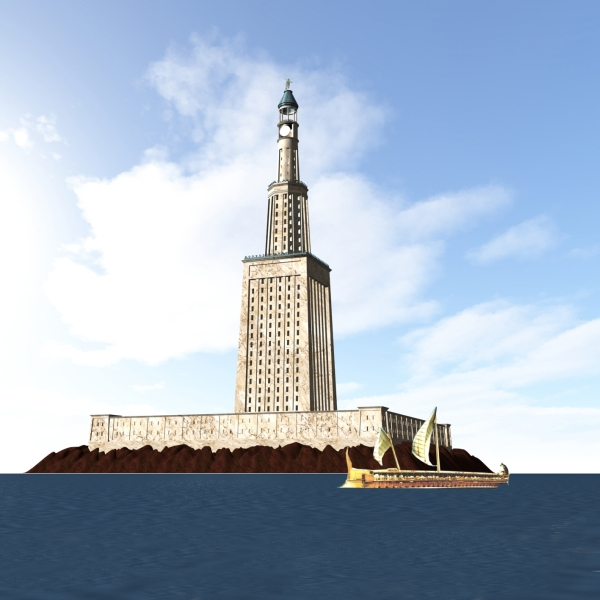
\includegraphics[width=\linewidth]{Imagenes/06.02.vor.imagenes/faro-alejandria.jpg}
  \caption{El faro de Alejadr\'ia {\small (reconstrucci\'on)} \\}
  \label{fig:faro.alejandria}
\end{wrapfigure}

En función de cómo se emite la señal luminosa, los faros se clasifican en: Faro de luz fija, faro de destellos, faro de luz centelleante, faro de grupos de destellos, faro de grupos de ocultaciones, faro de luz alternativa. Según la potencia de luz emitida y la altura en metros sobre el nivel del mar se obtiene el alcance geográfico, que no más que la distancia máxima a la que se ve la luz que emite.

Los colores universalmente adoptados para emitir luz en los faros son el blanco, verde y rojo. Puede darse el caso, bajo ciertas condiciones atmosféricas, que la luz blanca o la verde adquieran un tono rosado.


El faro es un elemento célebre y útil desde la época de los Romanos, recordado es el faro de Alejandría e incluso esta civilización  supo construir en la entrada de los puertos torres sumamente altas que imitaban de alguna manera al mencionado Faro de Alejandr\'ia (Figura \ref{fig:faro.alejandria}). En el siglo XIX se produciría el gran salto de calidad de los faros con el invento del físico francés Agustin Fresnel. Actualmente los faros son operados a distancia y de manera automática.


El faro más antiguo que se encuentra en funcionamiento es el de la Torre de Hércules ubicado en la península de La Coruña, en Galicia; su alto es de 68 metros, data del siglo I y es el único faro romano en pie.

Volviendo al sistema VOR, la antena de la estaci\'on emite una se\~nal de radiofrecuencia VHF en todas direcciones, que es recibida por el equipo VOR de cualquier aeronave que se encuentre dentro del rango de alcance (max. unos 240 km) y tenga sintonizada la frecuencia de dicha estaci\'on (que puede variar de 108 a 118 MHz).

\begin{figure}[!b]
 \centering
 \subfigure[D-VOR/DME ground station. Identificaci\'on "PEK" (Beijing)]
   {
   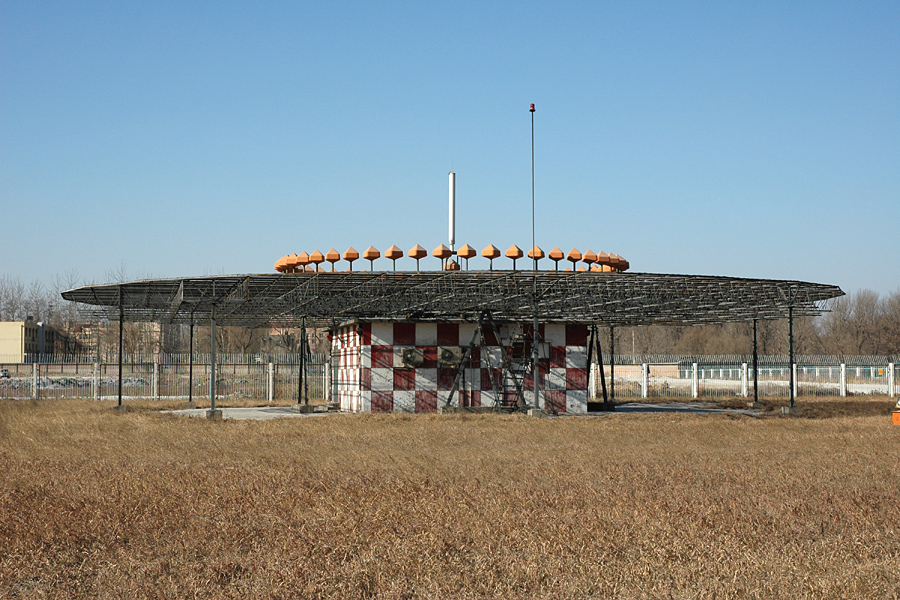
\includegraphics[height=5.5cm]{Imagenes/06.02.vor.imagenes/Vor_beijin.jpg}
   \label{fig:Vor_de_Beijin}
   }
 \subfigure[Esquema estaci\'on terrestre]
   {
   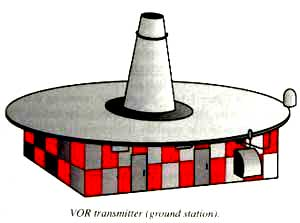
\includegraphics[height=5.5cm]{Imagenes/06.02.vor.imagenes/VORGroundStation.jpg}
   \label{fig:Vor.estacion.terrestre}
   }
 \caption{Estaciones VOR }
\end{figure}


La estaci\'on de tierra posee un diagrama de radiaci\'on din\'amico, transmite dos se\~nales VHF en el rango anteriormente mencionado. La radiofrecuencia emitida por un VOR lleva tres se\~nales codificadas. Una es la identificaci\'on de la estaci\'on en c\'odigo Morse \footnote{El c\'odigo Morse es un sistema de representaci\'on de letras y n\'umeros mediante se\~nales emitidas de forma intermitente.}, que permite al piloto saber de cu\'al estaci\'on se trata. Las otras dos son ondas senoidales de 30 Hz cuyas fases var\'ian entre si. Se les llama se\~nal de referencia y se\~nal variable respectivamente. La referencia mantiene siempre su fase constante, mientras que la variable cambia su fase seg\'un la direcci\'on en la que sea emitida. Dicha direcci\'on se mide como un azimut, es decir, se divide en 360 grados alrededor de la antena VOR contando en sentido horario a partir del norte magn\'etico terrestre, punto en el cual la se\~nal de referencia y la variable tienen fase id\'entica. De esta manera se puede visualizar una antena VOR como el punto desde el cual parten 360 l\'ineas de direcci\'on, a las que se les llama radiales.

El equipo VOR en la aeronave recibe la se\~nal VOR y decodifica sus tres se\~nales. Compara la se\~nal de referencia con la variable y determina la diferencia de fase entre las dos. De esta manera puede conocerse en qu\'e radial del VOR sintonizado se encuentra la aeronave con respecto al norte magn\'etico terrestre.

El VOR se utiliza en la aeron\'autica para navegar seg\'un el vuelo IFR \footnote{Recibe el nombre de Reglas de Vuelo Instrumental (m\'as conocido por sus siglas en ingl\'es, IFR), el conjunto de normas y procedimientos recogidos en el Reglamento de Circulaci\'on A\'erea, que regulan el pilotaje de aeronaves en condiciones de visibilidad reducida. Se trata del m\'etodo de navegaci\'on alternativo a las Reglas de Vuelo Visual o VFR.}, siempre permaneciendo en radio con un CTA. Los VOR suelen ir acompa\~nados de DME (Distance Measurement Equipment, Equipo de Medici\'on de Distancia), \'estos son completamente independientes del sistema VOR y ayudan al piloto a saber la distancia que hay entre la aeronave y la estaci\'on VOR. El VOR \'unicamente se utiliza en la llamada "radio navegaci\'on" por lo que siempre hay unos procedimientos que seguir que los marca la carta aeron\'autica para dirijirse a un VOR. Por ejemplo en las SID o salidas normalizadas de un aeropuerto, en la respectiva carta se verifica el procedimiento de apoyo en la salida con los NDB y VOR para poderla realizar correctamente. El piloto debe saber volar bajo reglas de vuelo IFR a un VOR y desde un VOR, o cualquier radioayuda que sea: (NDB, VOR, ILS u otras como el TACAN \footnote{Las siglas TACAN significan  TACtical Air Navigation,  es un tipo de ayuda a la navegaci\'on de uso militar.}) \cite{VOR-Wikipedia}.

Desarrollado de un sistema anterior, Visual-Aural Range (VAR), el VOR se dise\~n\'o para proveer 360 rumos desde y hacia la estaci\'on seleccionada por el piloto. Los antiguos transmisores de tubo de vac\'io con antenas rotadas mec\'anicamente se instalaron por todos lados en la d\'ecada de 1950 y en la de 1960 comenzaron a ser reemplazados por unidades de estado s\'olido. En este mismo per\'iodo se transformaron en el mayor sistema de navegaci\'on cuando reemplazaron a las viejas radiobalizas. Algunas de estas sobrevivieron como balizas no direccionales de baja o media frecuencia (NDB \footnote{Una Baliza No Direccional,  Non-Directional Beacon (NDB), es una estaci\'on de radio ubicada en un lugar conocido, utilizada como una ayuda para la navegaci\'on a\'erea o naval. Como su nombre implica, la se\~nal no provee informaci\'on direccional en contraste con nuevos tipos de ayudas como VOR. La se\~nal de una NDB copia el contorno de la curvatura de la tierra por lo que puede ser recibida a distancias mayores en latitudes menores, lo que constituye una ventaja sobre el sistema VOR. Sin embargo, la se\~nal NDB es afectada por condiciones atmosf\'ericas, terreno monta\~nosos, refracci\'on costera y tormentas el\'ectricas, particularmente a grandes distancias. A\'un con la aparici\'on de los sistemas VOR y GPS (Global Positioning System), las NDBs contin\'uan siendo las ayudas de navegaci\'on m\'as ampliamente usadas en el mundo. Las NDBs operan en el rango de frecuencias de 190 kHz a 535kHz (aunque tienen frecuencias reservadas en el rango de 190 a 1750 kHz) y una portadora modulada entre  400 o 1020 Hz \cite{NDB}. Entre la informaci\'on transmitida por una NDB se tiene:

\begin{itemize}
 \item Identificaci\'on por c\'odigo Morse entre 400 a 1020 Hz.
\item Informaci\'on de la Terminal A\'erea (Airfield Terminal Information Service = ATIS)
\item Servicio de informaci\'on clim\'atica de la Terminal A\'erea (Airfield Weather Information Service = AWIS), o, en una emergencia un controlador de tr\'afico a\'ereo activando la funci\'on de Presionar-para-hablar (Press-To-Talk = PTT), puede modular la portadora con la voz. El piloto utiliza su receptor ADF para escuchar las instrucciones desde la torre.
\end{itemize}
}).

En los aviones de hoy en d\'ia esto se realiza mediante la FMC, o MCDU seg\'un el fabicante del avi\'on, ya que intoducen directamente la SID y la FMC la realiza automaticamente sola. As\'i podemos llevar a cabo un vuelo, tanto de larga como de corta distancia entre dos puntos del mundo.

En las rutas a\'ereas comerciales m\'as transitadas, al igual que en las carreteras terrestres, hay cruces y curvas. Bajo estos "cruces" y "curvas" se suelen instalar estas estaciones VOR. Las "carreteras a\'ereas" son los radiales de XXX grados que parten de un VOR y que normalmente llegan a otro VOR o incluso a una pista de aterrizaje.

El piloto puede ordenar al piloto autom\'atico: "\textit{Sigue el radial de 115 grados del VOR que transmite en la frecuencia 109.75 Mhz}.", y el avi\'on autom\'aticamente, cuando se cruce con el radial 115, lo seguir\'a hasta sobrevolar el VOR.

\begin{figure} [ht]
 \centering
 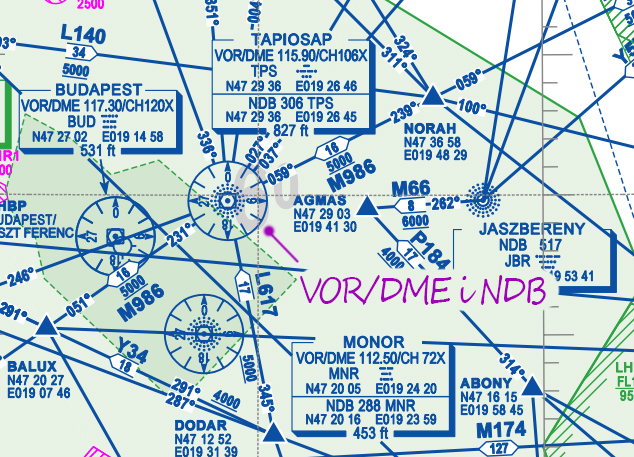
\includegraphics[width=0.9\textwidth,bb=0 0 500 301]{Imagenes/06.02.vor.imagenes/mapa_vor.jpg}
 % Mapa_VOR.eps: 0x0 pixel, 300dpi, 0.00x0.00 cm, bb=0 0 500 301
 \caption{Mapa con ruta y posici\'on de estaciones VOR}
 \label{Mapa_estaciones_VOR}
\end{figure}

En el mapa de la Figura  \ref{Mapa_estaciones_VOR} se puede ver una serie de radiobalizas VOR (los c\'irculos grandes) interconectadas entre si por rutas a\'ereas. Cada ruta a\'erea tiene marcado su nombre, altitud y rumbo (que coincide con el radial del VOR del que parte).


